\documentclass[a4paper,titlepage]{scrartcl}
\pagestyle{plain}
\usepackage[utf8]{inputenc}
\usepackage[T1]{fontenc}
\usepackage[german]{babel}
\usepackage{float}
\usepackage{graphicx}
\usepackage{amsmath,amssymb,amstext,tabularx}
\usepackage{enumerate}
\usepackage{units}
\usepackage{mhchem, numprint,caption,rotating,longtable}
\newcommand{\angstrom}{\mbox{\normalfont\AA}}
\numberwithin{equation}{section}
\renewcommand{\sc}{\textsc}

\title{Strukturbestimmung aus Pulverdiagrammen}
\author{Genti Saliu\\Gruppe 106}
\date{Versuchstag: 15. Dezember 2014}

\begin{document}
	\begin{titlepage}
		\maketitle
		\thispagestyle{empty}
	\end{titlepage}
	
\newpage
\pagenumbering{roman}
\tableofcontents

\newpage
\pagenumbering{arabic}

\section{Ziel des Versuchs}
Ziel dieses Versuchs ist es mit dem Verfahren nach Debye-Scherrer die Strukturanalyse eines Kupferkristalls durchzuführen. Es sollen dabei u.a. die Millersche-Indizes $hkl$, Gitterkonstante, Bravais-Gitter, Strukturfaktor und Atomabstände bestimmt werden.
\section{Theoretische Grundlagen}
\subsection{Kristalliner Zustand \cite{kittel}, \cite{wiki:kristallstruktur}}
\subsubsection{Kristallstruktur}
Ein (idealer) Kristall entsteht durch die unendliche Wiederholung identischer Atomgruppen. Diese Atomgruppe wird Basis genannt und stellt die kleinste Gruppe dar, die sich periodisch im dreidimensionalen Raum wiederholt. Sie kann aus eins bis einige tausent Atomen, Ionen oder Molekülen bestehen.\\ \\
Jeder Basis wird ein Bezugspunkt zugewiesen, diese Punkte bilden das \emph{Kristallgitter}. Davon werden Basisvektoren aufgespannt, die von diesem Gitterpunkt zu seinen Nachbarn weisen. Das Parallelepiped, das von diesen Basisvektoren $\vec{a_i}$ aufgespannt wird,  heißt Einheits- oder \emph{Elementarzelle}. Die Seitenlänge $a$ der Elementarzelle nennt man Gitterkonstante. Die Elementarzelle mit dem kleinsten Volumen nennt man \emph{primitive Elementarzelle}. In jeder primitiven Elementarzelle gibt es genau einen Gitterpunkt.
\begin{figure}[H]
	\centering
	\begin{tabular}{@{}r@{}}
		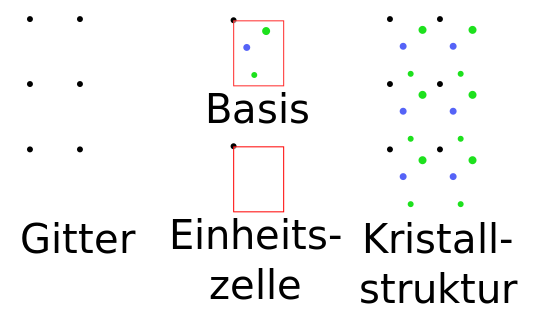
\includegraphics[width=0.5\textwidth]{kristallstruktur.png}\\
		\footnotesize\sffamily\textbf{Quelle:} Wikipedia \cite{wiki:kristallstruktur}
	\end{tabular}
	\caption{Kristallstruktur}
    \label{fig:kristallstruktur}
\end{figure}
Gitter und Basis stellen eine Kristallstruktur dar. Mit der \emph{Koordinationszahl} $KZ$ gibt man die Anzahl der nächsten Nachbarn einer Struktureinheit (Atom, Ion, Molekül) an.\\ \\
Die Verschiebung des Kristalls parallel zu sich selbst um einen Translationsvektor $\vec{T}$ nennt man Gittertranslation:
\begin{equation*}
\vec{T}=u_1 \vec{a}_1 + u_2 \vec{a}_2 + u_3 \vec{a}_3
\end{equation*}
$\vec{a}_1$, $\vec{a}_2$ und $\vec{a}_3$ sind primitive Translationsvektoren - es gibt im Kristall keine Zelle mit kleinerem Volumen als $\vec{a}_1 \cdot \vec{a}_2 \times \vec{a}_3$, das ist das Volumen der primitiven Elementarzelle. Primitive Translationsvektoren werden zur Definition der \emph{Kristallachsen} benutzt.\\ \\
\subsubsection{Reziprokes Gitter}
Neben dem oben vorgestellten Punktgitter im Ortsraum, definiert man ein Punktgitter im \emph{reziproken Raum}, auch genannt \emph{reziprokes Gitter}, das durch die Vektoren $\vec{b_i}$ aufgespannt wird:
\begin{equation*}
b_i=\frac{2 \pi}{V_{EZ}} a_j \times a_k
\end{equation*}
mit $V_{EZ}$ das Volumen der Einheitszelle. Der Translationsvektor im reziproken Gitter sieht dann wie folgt aus:
\begin{equation*}
\vec{G}=\sum_{i=1}^3 h_i b_i \quad \quad \text{mit} \quad h_i=0, \pm 1, \pm 2, ...
\end{equation*}
Im dreidimensionalen Raum:
\begin{equation*}
\vec{G}=h \vec{b}_1+k \vec{b}_2+l \vec{b}_3
\end{equation*}
\subsubsection{Kristallebenen und Millersche Indizes \cite{wiki:miller}, \cite{kittel}}
Die Millerschen Indizes geben die Lage einer Kristallebene an, die durch drei beliebige, nicht kollineare Punkte in den Kristallachsen festgelegt ist. Das sind die Schnittpunkte der Ebene mit den Kristallachsen (Abbildung \ref{fig:miller}).
\begin{figure}[H]
	\centering
	\begin{tabular}{@{}r@{}}
		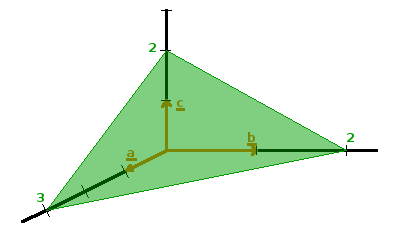
\includegraphics[width=0.5\textwidth]{bravaismiller.png}\\
		\footnotesize\sffamily\textbf{Quelle:} Aberystwyth University \cite{miller}
	\end{tabular}
	\caption{Kristallebene schneidet die Kristallachsen}
    \label{fig:miller}
\end{figure}
Im Ortsraum kann man die Millerschen Indizes so bestimmen:
\begin{itemize}
\item Bestimme die Schnittpunkte $s_1 \vec{a}_1$, $s_2 \vec{a}_2$, $s_3 \vec{a}_3$ der Ebene mit den Achsen $\vec{a}_1$, $\vec{a}_2$, $\vec{a}_3$ in Einheiten der Gitterparameter $a_1$, $a_2$, $a_3$.
\item Bilde den zur Ebene Normalenvektor $\vec{n}$:
\begin{equation*}
\vec{n}=\begin{pmatrix}\frac{1}{s_1}\\\frac{1}{s_2}\\\frac{1}{s_3}\end{pmatrix}
\end{equation*}
\item Bilde ein Vielfaches $j$ des Normalenvektors, sodass alle Komponenten dieses Vielfachen des Normalenvektors ganze teilerfremde Zahlen sind:
\begin{equation*}
\vec{n}_1=\begin{pmatrix}\frac{j}{s_1}\\\frac{j}{s_2}\\\frac{j}{s_3}\end{pmatrix}=\begin{pmatrix}h\\k\\l\end{pmatrix}
\end{equation*}
Die Komponenten des Tupels $(hkl)$ sind die Millerschen Indizes.\\ \\
Schneidet die Ebene eine Achse auf der negativen Seite des Ursprungs, so ist der zugehörige Index negativ und wird über ein Minuszeichen über dem Index kenntlich gemacht, z.B. $(h\overline{k}l)$.
\end{itemize}
Im reziproken Raum wird anhand den Millerschen Indizes $(hkl)$ der Vektor
\begin{equation*}
\vec{G}=h \vec{b}_1+k \vec{b}_2+l \vec{b}_3
\end{equation*}
bezeichnet, der senkrecht auf den entsprechenden Gitterebenen steht. Dabei haben die Zahlen $h$, $k$, $l$ keinen gemeinsamen Teiler.\\ \\
Weil die Gittervektoren des reziproken Raumes senkrecht auf den Netzebenen (Gitterebenen) im Ortsraum stehen, können die Millerschen Indizes zur Bestimmung des Ebenenabstandes benutzt werden:
\begin{equation*}
d_{hkl}=\frac{2 \pi}{|\vec{G}_{hkl}|}
\end{equation*}
\subsubsection{Gittervektoren}
Vektoren können ebenfalls durch Indizes bezeichnet werden. Dabei werden eckige Klammern verwendet $[uvw]$:
\begin{equation*}
u\vec{a}_1+v\vec{a}_2+w\vec{a}_3
\end{equation*}
\subsection{Symmetrie von Kristallen}
Kristalle können durch Symmetrieoperationen in sich selbst überführt werden. Mögliche Symmetrioperationen sind \cite{kittel}:
\begin{itemize}
\item Translation
\begin{equation*}
\vec{T}=n_1\vec{a}_1+n_2\vec{a}_2+n_3\vec{a}_3
\end{equation*}
\item Drehungen um eine Achse, die durch einen Gitterpunkt geht. Es können nur ein-, zwei-, drei-, vier- oder sechszählige Drehachsen existieren, die Drehungen um die Winkel $2\pi$, $\frac{2\pi}{2}$, $\frac{2\pi}{3}$, $\frac{2\pi}{4}$, $\frac{2\pi}{6}$ und deren ganzzahligen Vielfachen entsprechen.
\item Spiegelungen an einer Ebene durch einen Gitterpunkt
\item Inversion bzw. Drehung um $\unit[180]{^\circ}$ gefolgt von einer Spiegelung an einer Ebene senkrecht zur Drehachse
\end{itemize}
\emph{Raumgruppen} beschreiben im dreidimensionalen Raum die Symmetrien des Kristalls. Neben den oben erwähnten Symmetrien sind auch Translationen in Form von Schraubungen und Gleitspiegelungen sowie Kombinationen davon möglich. Fasst man das Hintereinanderausführen von Symmetrieoperationen als multiplikative Verknüpfung auf, so ist die Menge von Symmetrieoperationen eine Gruppe. \\ \\
Empirisch sind in drei Dimensionen 230 mögliche Raumgruppen für Kristalle bestimmt worden. Die Raumgruppen werden in 7 Kristallsysteme, 14 Bravaisgitter und 32 Kristallklassen eingeteilt. \cite{wiki:raumgruppe} \\ \\
\emph{Kristallsysteme} sind ein Klassifizierungsschema für Kristalle in drei Dimensionen, sie stellen die Parallelepipede eines Gitters dar. Die 7 Kristallsysteme sind triklin, monoklin, orthorhombisch, tetragonal, trigonal, hexagonal und kubisch.\\ \\
Bravaisgitter bezeichnet die Menge aller im zwei- oder dreidimensionalen Raum möglichen Einheitszellen der Kristalle, wo
\begin{itemize}
\item die Einheitszelle die einfachste sich wiederholende Einheit im Kristall ist
\item gegenüberstehende Flächen der Einheitszelle parallel sind
\item der Rand der Einheitszelle äquivalente Stellen verbinden
\end{itemize}
\cite{bravais}\\ \\
Die Differenzierung der Kristallsysteme zu den 14 Bravais-Gittern erfolgt durch Anordungung weiterer Gitterpunkte, entweder in der Raummite (raumzentriert), auf den Mittelpunkten aller Begrenzungsflächen (flächenzentriert) oder auf den Mittelpunkten der zwei Basisflächen (basiszentriert) der Elementarzelle. \cite{bravais}\\ \\
Streicht man in einer Raumgruppe alle Translationen und ersetzt zusätzlich die Schraubenachsen und Gleitspiegelebenen durch entsprechende Drehachsen und Spiegelebenen, so erhält man die \emph{geometrische Kristallklasse} oder \emph{Punktgruppe} des Kristalls. Als Kristallklassen kommen nur solche Punktgruppen in Frage, bei deren Symmetrie das Gitter invariant bleibt. \cite{wiki:punktgruppe}
\subsection{Dichteste Kugelpackungen \cite{wiki:kugelpackung} \cite{vorbereitungsMappe} \cite{kittel}}
Eine dichteste Kugelpackung ist die geometrische Anordnung unendlich vieler Kugeln gleicher Größe im 3-dimensionalen Raum so, dass diese einander nur berühren und nicht überlappen und dabei den verbleibenden Leerraum minimal lassen. Die Packungsdichte einer dichtesten Kugelpackung beträgt:
\begin{equation*}
\frac{\pi}{3 \sqrt{2}}\approx\unit[74]{\%}
\end{equation*}
Im Modell der Kugelpackungen werden Atome bzw. Ionen als annährend starre Kugeln betrachtet.
\subsubsection{Struktur}
Eine dichteste Kugelpackung beruht auf die Stapelung dicht gepackter hexagonaler Schichten, in denen eine Kugel jeweils von sechs Nachbarkugeln umgeben ist. Durch die Stapelung einer zweiten hexagonalen Schicht auf die erste entsteht eine dichte Packung, wenn die Kugeln der zweiten Schicht in die Lücken der ersten einrasten. Jede Schicht besitzt zwei Arten von Lücken, eine mit der Spitze nach unten und eine mit der Spitze nach oben.\\ \\
Bezeichnet man die Lagen der Kugeln in einer Schicht mit $A$ und die beiden Lückenarten mit $B$ und $C$,  so können die Kugeln $A$ einer zweiten Schicht entweder in die Lücken $B$ oder $C$ einrasten. Bei einer dritten Schicht kann sie entweder die Lage $C$ oder $A$ bzw. $B$ oder $A$ einnehmen, falls die zweite Schicht die Lage $B$ bzw. $C$ besetzt.
\subsubsection{Hexagonal und kubisch dichteste Kugelpackung}
Es gibt unendlich viele Möglichkeiten dichteste Kugelpackungen aufzubauen, die zwei wichtigsten sind:
\begin{itemize}
\item \textbf{die hexagonal dichteste Kugelpackung} (''hcp'' bzw. ''hexagonal close packing'') besitzt die Stapelfolge $ABABAB...$ bzw. $ACACAC...$, die übernächste Schicht nimmt wieder die Lage der Ausgangsschicht ein, somit beträgt die Periodenlänge zwei Schichten. Die entstehende Struktur hat eine hexagonale Symmetrie mit Achsenverhältnis $\frac{c}{a}=\sqrt{\frac{8}{3}}=1.633$, wobei $a$ in der Basisebene und $c$ senkrecht dazu liegen (s. Abbildung \ref{fig:hexagonalkugel}).
\item \textbf{die kubisch dichteste Kugelpackung} (''ccp'' bzw. ''cubic close packed'') besitzt die Stapelfolge $ABCABC...$ bzw. $ACBACB$, die Periodenlänge beträgt drei Schichten.
\end{itemize}
\begin{figure}[H]
	\centering
	\begin{tabular}{@{}r@{}}
		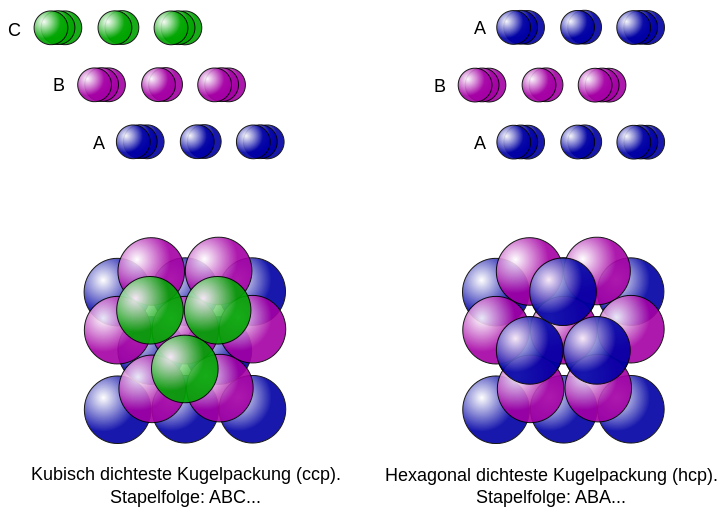
\includegraphics[width=0.55\textwidth]{DichtesteKugelpackung.png}\\
		\footnotesize\sffamily\textbf{Quelle:} Wikipedia \cite{wiki:kugelpackung}
	\end{tabular}
	\caption{Kubisch dichteste Kugelpackung (ccp) und hexagonal dichteste Kugelpackung (hcp)}
    \label{fig:dichtestepackung}
\end{figure}
\begin{figure}[H]
\centering
	\begin{tabular}{@{}r@{}}
		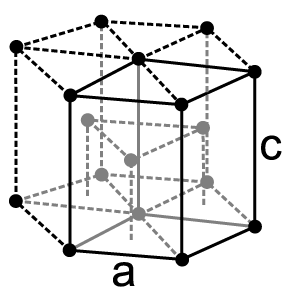
\includegraphics[width=0.4\textwidth]{hexagonalkugelpackung.png}\\
		\footnotesize\sffamily\textbf{Quelle:} Wikipedia
	\end{tabular}
	\caption{Hexagonal dichteste Kugelpackung (hcp) mit Achsen $c$ und $a$}
    \label{fig:hexagonalkugel}
\end{figure}
\subsubsection{Oktaeder- und Tetraederlücken}
Wir sahen, dass bei der dichtesten Kugelpackung eine Raumerfüllung von $\unit[74]{\$}$ vorliegt, der restliche $\unit[26]{\%}$ wird von Tetraeder- und Oktaederlücken besetzt.\\ \\
Die Oktaederlücke ist der Hohlraum, der von sechs benachbarten Atomen oder Ionen in zwei Schichten gebildet wird.  Der Name kommt daher, dass die Atome einen Oktaeder bilden.\\ \\
Bei der kubisch dichtesten Kugelpackung (Abbildung \ref{fig:oktaeder}) liegt eine Lücke in der Mitte der Elementarzelle und 12 weitere auf den Kantenmitten. Da die Lücken auf den Kantenmitten mit je vier benachbarten Elementarzellen geteilt werden, beträgt die Gesamtanzahl der Oktaederlücken pro Elementarzelle $1 + 12 \cdot \frac{1}{4}=4$.\\ \\
Bei der hexagonal dichtesten Kugelpackung befinden sich die Oktaederlücken senkrecht übereinanderliegend auf den Positionen $(\frac{1}{3},\frac{2}{3},\frac{1}{4})$ und $(\frac{1}{3},\frac{2}{3},\frac{3}{4})$.\\ \\
Die Größe der Oktaederlücke kann durch den Radius $r$ der größten Kugel angegeben werden, die in die Lücke hineinpasst. Man erhält dafür:
\begin{equation*}
r=(\sqrt{2}-1)R\approx 0.414 \cdot R
\end{equation*}
wobei $R$ der Radius der großen Kugeln in den Ecken des Oktaeders ist.
\begin{figure}[H]
\centering
\begin{minipage}{.4\textwidth}
	\centering
  	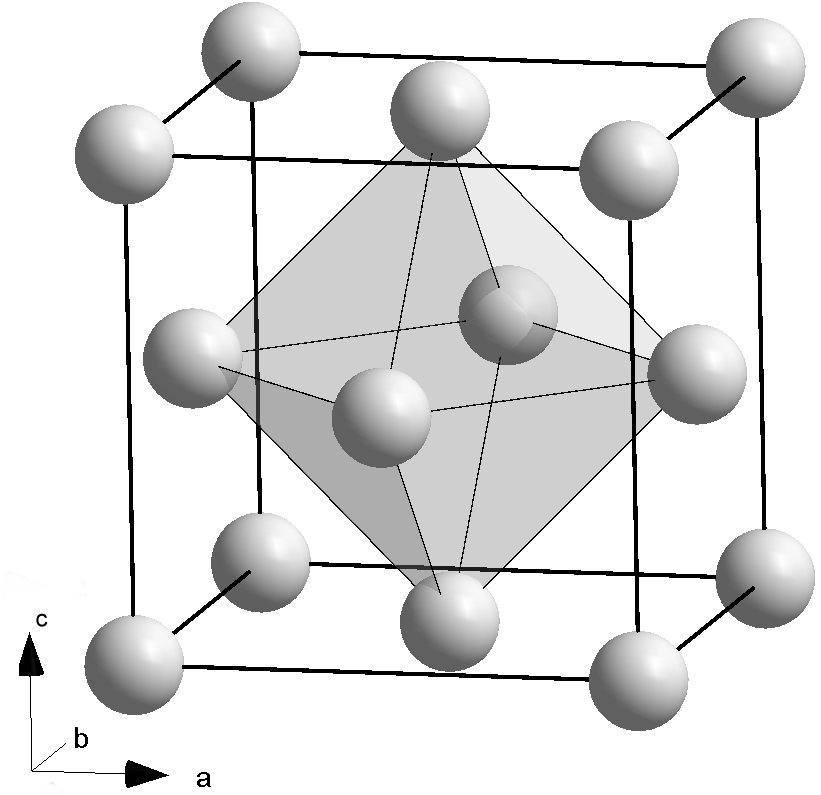
\includegraphics[width=0.9\textwidth]{oktaeder.png}\\
	\footnotesize\sffamily\textbf{Quelle:} Wikipedia \cite{wiki:oktaederluecke}
    \captionsetup{width=\textwidth}
	\captionof{figure}{Oktaederlücke in einer kubisch-dichtesten Kugelpackung}
    \label{fig:oktaeder}
\end{minipage}%
\begin{minipage}{.4\textwidth}
	\centering
	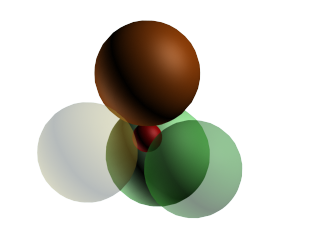
\includegraphics[width=0.9\textwidth]{tetraeder.png}\\
	\footnotesize\sffamily\textbf{Quelle:} Wikipedia \cite{wiki:tetraederluecke}
	\captionsetup{width=\textwidth}
	\captionof{figure}{Tetraederlücke}
	\label{fig:tetraeder}
\end{minipage}
\end{figure}
Die Tetraederlücke ist der Hohlraum, der von vier benachbarten Atomen oder Ionen in zwei Schichten gebildet wird.\\ \\
Bei der kubisch dichtesten Kugelpackung befinden sie sich in den Mitten der Achtelwürfeln auf den Positionen $(\frac{1}{4},\frac{1}{4},\frac{1}{4})$, $(\frac{1}{4},\frac{1}{4},\frac{3}{4})$, $(\frac{1}{4},\frac{3}{4},\frac{1}{4})$, $(\frac{3}{4},\frac{1}{4},\frac{1}{4})$, $(\frac{1}{4},\frac{1}{4},\frac{3}{4})$, $(\frac{3}{4},\frac{1}{4},\frac{3}{4})$, $(\frac{3}{4},\frac{3}{4},\frac{1}{4})$ und $(\frac{3}{4},\frac{3}{4},\frac{3}{4})$.\\ \\
Bei der hexagonal dichtesten Kugelpackung befinden sich tetraedrische Lücken auf den Positionen $(0,0,\frac{3}{8})$,$(0,0,\frac{5}{8})$,$(\frac{2}{3},\frac{1}{3},\frac{1}{8})$ und $(\frac{2}{3},\frac{1}{3},\frac{7}{8})$.\\\\
Auch hier wird die Größe der Tetraederlücke durch den Radius $r$ der größten Kugel angegeben, die in die Lücke hineinpasst:
\begin{equation*}
r=\frac{1}{2}(\sqrt{6}-2) \cdot R\approx0.22478 \cdot R
\end{equation*}
\subsubsection{Strukturtypen mit dichtester Kugelpackung \cite{wiki:kugelpackung}}
\begin{description}
\item[Einatomige Systeme] \hfill \\
Die Struktur vieler Metalle entspricht einer dichtesten Kugelpackung, wobei am häufigsten die hexagonal und kubisch dichteste Kugelpackung vorkommen. Da es unendlich viele Schichtfolgen gibt, existieren damit auch unendlich viele verschiedene dichteste Kugelpackungen.\\ \\
Der Strukturtyp hexagonal dichteste Kugelpackung mit Schichtfolge $ABABAB...$ hat die Nummer $A3$ und wird auch Magnesium-Typ genannt. Diesem Strukturtyp gehören u.a. Berllium, Scandium und Titan.\\\\
Der Strukturtyp kubisch dichteste Kugelpackung mit Schichtfolge $ABCABC...$ hat die Nummer $A1$ und wird auch Kupfer-Typ genannt. Dazu gehören Kupfer, Silber und Gold.\\ \\
Bestimmte Metalle nehmen noch eine weitere dichteste Kugelpackung mit Schichtfolge $ABACABAC...$ an, die derselben Raumgruppe wie $hcp$ gehört, aber vier Atome in der Elementarzelle hat. Dieser Strukturtyp wird \emph{double hexagonal closed packed} (dhcp) genannt.
\item[Mehratomige Systeme] \hfill \\
Bei vielen Kristallstrukturen mit ionischem Bindungstyp kommt es zu einer dichtesten Kugelpackung eines Teils der Ionen und der Einlagerung der anderen Ionen in den Lücken. Falls die Einlagerungsionen in die Lücke nicht hineinpassen, wird die Kugelpackung deformiert, deren Art und Ausmaß vom Größenverhältnis der Ionen zu den Einlagerungsionen abhängen.
\item[Polytype] \hfill \\
Polytype sind Kristalle mit Stapelfolgen, die eine lange Wiederholungseinheit haben. Diese Polytype verfügen zum Teil über extrem große Gitterkonstanten. Beispiele sind Zinksulfid (\ce{ZnS}) und Siliciumcarbid (\ce{SiC}).
\end{description}
\subsection{Röntgenstrahlung \cite{wiki:roentgenstrahlung} \cite{vorbereitungsMappe} \cite{wiki:roentgenstrahlung} \cite{wiki:bremsstrahlung} \cite{wiki:charakteristischeStrahlung}}
\subsubsection{Einführung}
Röntgenstrahlen sind elektromagnetische Wellen mit Photoenergien zwischen $\unit[100]{eV}$ und einigen $\unit{MeV}$ und entsprechenden Wellenlängen zwischen $\unit[10^{-8}]{m}$ und $\unit[10^{-12}]{m}$.\\ \\
In diesem Versuch und u.a. in der Kristallographie wird die Beugung von Röntgenstrahlen in Kristallen zu deren Strukturbestimmung benutzt.\\ \\
Für die Angabe der Wellenlänge werden wir durchgehend die Einheit Ångström ($\angstrom$) verwenden:
\begin{equation*}
\unit[1]{\angstrom}=\unit[100]{pm}=\unit[10^{-10}]{m}
\end{equation*}
\subsubsection{Erzeugung von Röntgenstrahlen}
Röntgenstrahlen entstehen durch:
\begin{itemize}
\item starke Beschleunigung geladener Teilchen (meistens Abbremsung oder Ablenkung von Elektronen)
\item hochenergetische Übergänge in den Elektronenhüllen von Atomen oder Molekülen
\end{itemize}
Diese Röntgenstrahlen nennt man jeweils (weiße) Brems- bzw. charakteristische Strahlung (Eigenstrahlung). Bremsstrahlung weist ein kontinuierliches Spektrum, charakteristische Strahlung ein Linienspektrum auf.\\ \\
Sie können mit der Röntgenröhre oder dem Synchroton erzeugt werden, die beide dieser Effekte ausnutzen. Wir erklären im Folgenden die Funktionsweise der Röntgenröhre.\\ \\
Bei der Röntgenröhre werden Elektronen zunächst von der Kathode aus durch ein elektrisches Feld beschleunigt und treffen anschließend auf die Anode auf, wo sie stark abgebremst werden. Es entsteht Röntgenstrahlung (Bremsstrahlung).\\ \\
Ausserdem werden durch Elektronenstöße Elektronen aus den Schalen der Metallatome herausgeschlagen. Die entstandenen Löcher in den Schalen werden durch andere Elektrone aufgefüllt, wodurch es zur charakteristischen Röntgenstrahlung kommt.\\ \\
Die minimale Wellenlänge der Bremsstrahlung $\lambda_{min}$ hängt nicht vom Anodenmaterial, sondern nur von der Beschleunigungsspannung $U$ ab:
\begin{equation*}
\lambda_{min}=\frac{h \cdot c}{e \cdot U}
\end{equation*}
wobei $h$ das Plancksche Wirkungsquantum, $c$ die Lichtgeschwindigkeit, $e$ die Elementarladung und $U$ die Beschleunigungsspannung sind.\\ \\
Die Intensität der Bremsstrahlung hängt von der Beschleunigungsspannung $U$ und der Ordnungszahl $Z$ des Anodenmaterials:
\begin{equation*}
J(\lambda)=K \cdot I \cdot Z \cdot \left( \frac{\lambda}{\lambda_{min}} - 1 \right) \cdot \frac{1}{\lambda^2}
\end{equation*}
wobei $J$ die Intensitätsfunktion, $K$ die Kramersche Konstante, $I$ der Elektronenstrom und $Z$ die Ordnungszahl des Anodenmaterials sind.\\ \\
Die Eigenstrahlung ist für das Anodenmaterial charakteristisch. Die Linien ihres Spektrums beschreiben angeregte Niveauübergänge und werden $K_{\alpha}$, $K_{\beta}$ usw. genannt. Die Buchstaben $K$, $L$, $M$ usw. geben die innere Schale an, in die das Elektron bei der Emission übergangen ist, die griechische Buchstabe als Index gibt die Differenz zur Hauptquantenzahl $n$ der äußeren Schale an.
\subsubsection{Monochromatisierung}
Die von der Röntgenröhre emittierte Strahlung ist polychromatisch mit Strahlung verschiedener Wellenlängen.\\ \\
Um monochromatisierte Strahlen zu erhalten, werden Röntgenstrahlen an geeigneten Monochromatorkristallen gestreut, wobei winkelabhängig Strahlen bestimmter Wellenlängen bevorzugt werden.\\ \\
Monochromatisierung kann auch durch Filter mit Absorptionskanten zwischen den $K \alpha$- und $K \beta$-Linien realisiert werden.\\ \\
Monchromatisierte Röntgenstrahlen sind für das Debye-Scherrer-Experiment erforderlich.
\subsection{Geometrie der Röntgeninterferenzen \cite{roentgeninterferenzen}}
Wie schon besprochen, besteht eine Kristallstruktur aus einer 3-dimensional periodisch gitterhaften Atomanordnung. Dabei sind mit Röntgenstrahlung Interferenzeffekte zu beobachten.\\ \\
Sind $\vec{s}_0$ und $\vec{s}$ Einheitsvektoren in Richtung des einfallenden und des gestreuten Strahls, so beträgt die Wegdifferenz zwischen Strahlen, die am Ort $\vec{r}$ in Richtung $\vec{s}$ gestreut werden:
\begin{equation*}
g=(\vec{s}-\vec{s}_0) \cdot \vec{r}
\end{equation*}
Das entspricht einer Phasendifferenz
\begin{equation*}
\phi=\frac{2 \pi g}{\lambda}=2\pi \frac{\vec{s}-\vec{s}_0}{\lambda} \vec{r}=2 \pi \vec{S} \vec{r}
\end{equation*}
mit $\vec{S}=\frac{\vec{s}-\vec{s}_0}{\lambda}$ der Streuvektor.\\\\
Gibt es in einem Kristall ein Atom mit Ortsvektor $\vec{r}_0$, so gibt es identische Atome an den Orten
\begin{equation*}
\vec{r}=\vec{r}_0+u\vec{a}+v\vec{b}+w\vec{c}
\end{equation*}
die sich um Gittertranslationen
\begin{equation*}
\vec{t}=u \vec{a}+v \vec{b} + w \vec{c}
\end{equation*}
unterscheiden. Das elektrische Feld, das am Kristall gestreut wird, ergibt sich aus der Summe aller Atome in der Elementarzelle, die um alle Gittervektoren $\vec{t}=u \vec{a} + v \vec{b} + w \vec{c}$ verschoben sind:
\begin{align*}
E&=E_{th} \sum_j f_j e^{2 \pi i \vec{S} \vec{r}_j} \sum_u \sum_v \sum_w e^{2 \pi i \vec{S} (u \vec{a} + v \vec{b} + w \vec{c})}\\
&=E_{Th} \cdot F(\vec{S}) \cdot G(\vec{S})
\end{align*}
Dabei beschreibt $E_{Th}=-r_e \frac{E_0}{R} \cos{(2 \theta)}$ das an einem Elektron unter dem Winkel $2 \theta$ elastisch gestreute elektrische Feld.\\ \\
Der Term
\begin{equation}
\label{eq:strukturfaktor}
F(\vec{S})=\sum_j f_j e^{2 \pi i \vec{S} \vec{r}_j}
\end{equation}
ist der Strukturfaktor der Elementarzelle.\\ \\
Der Term
\begin{equation*}
G(\vec{S})=\sum_u e^{2 \pi i u \vec{S} \vec{a}} \sum_v e^{2 \pi i v \vec{S} \vec{b}} \sum_w e^{2 \pi i w \vec{S} \vec{c}}
\end{equation*}
verschwindet nur dann nicht, wenn die Laue Bedingungen erfüllt sind:
\begin{figure}[H]
\begin{minipage}{.5\linewidth}
\begin{align*}
\vec{S} \cdot \vec{a}&=h\\
\vec{S} \cdot \vec{b}&=k\\
\vec{S} \cdot \vec{c}&=l
\end{align*}
\end{minipage}
\text{bzw.}
\begin{minipage}{.5\linewidth}
\begin{align*}
(\vec{s}-\vec{s}_0) \cdot \vec{a}&=h \cdot \lambda \\
(\vec{s}-\vec{s}_0) \cdot \vec{b}&=k \cdot \lambda \\
(\vec{s}-\vec{s}_0) \cdot \vec{c}&=l \cdot \lambda
\end{align*}
\end{minipage}
\caption*{Laue Bedingungen}
\end{figure}
Die Laue-Bedingungen besagen, dass man dann eine konstruktive Interferenz erhält, wenn der Streuvektor $\vec{S}=\frac{\vec{s}-\vec{s}_0}{\lambda}$ beim Streuen mit einem reziproken Gittervektor $\vec{H}=h \vec{a}^*+k \vec{b}^* + l \vec{c}^*$ zusammenfällt:
\begin{equation*}
\frac{\vec{s}-\vec{s}_0}{\lambda}=\vec{S} \equiv \vec{H}=h \vec{a}^*+k \vec{b}^* + l \vec{c}^*
\end{equation*}
Für alle anderen Streuvektorenwird $F(\vec{S})=0$. $h$, $k$, $l$ sind die Millerschen Indizes der Netzebenen mit Abstand $d=\frac{n}{| \vec{H} |}$, wobei $n$ die Beugungsordnung ist.\\ \\
Aus $|\vec{H}|=|\vec{S}|=2 \sin{(\frac{\theta}{\lambda})}$ und $|\vec{H}|=\frac{n}{d}$ folgt die Braggsche Gleichung:
\begin{equation*}
n \cdot \lambda = 2d \sin{\theta}
\end{equation*}
die als skalare Form der Laue-Gleichungen anzusehen ist. Sie hat praktische Bedeutung bei der Interpretation der Beugung und Interferenz einer ebenen Röntgenwelle an kristallinen Festkörpern formal als Reflexion der Röntgenstrahlung an Scharen paralleler Atomebenen interpretieren. Die an den Atomen einer solchen Ebene gestreuten Wellen addieren sich genau phasengleich, wenn für den in der Richtung $\vec{s}_0$ einfallenden Strahl und den in der Richtung $\vec{s}$ reflektierten Strahl die Reflexionsbedingung
\begin{equation*}
\vec{s}-\vec{s}_0=\lambda \cdot \vec{H}
\end{equation*}
erfüllt ist.\\ \\
Aus den Wellenvektoren $\vec{K}=\frac{2 \pi \vec{s}}{\lambda}$ und $\vec{K}_0=\frac{2 \pi \vec{s}_0}{\lambda}$ folgt die Laue-Gleichung:
\begin{equation*}
\vec{K}-\vec{K}_0=2 \pi \vec{H}
\end{equation*}
Die Laue-Gleichung lässt sich mithilfe der Ewald-Kugel bzw. Ewald-Konstruktion geometrisch darstellen. Die Konstruktion verknüpft dabei den realen und den reziproken Raum und wird benutzt, um die möglichen Beugungsrichtungen des Röntgenstrahls beim Auftreffen auf den Kristall zu bestimmen.
\subsection{Intensität der Röntgeninterferenzen \cite{roentgenbeugung} \cite{roentgeninterferenzen} \cite{wiki:ausloeschung}}
Die Intensität der Röntgeninterferenzen beträgt
\begin{equation}
\label{eq:intensitaetpunkt}
I=\left( \frac{e^2}{mc^2} \right)^2 \cdot \frac{1}{r_a^2} \cdot \left( \frac{1 + \cos^2{2 \theta}}{2} \right) \cdot I_0 \cdot |F(\vec{H})|^2 \cdot N_1^2 N_2^2 N_3^2
\end{equation}
mit $I_0$ die ursprüngliche Intensität der Röntgenstrahlen, $N_1$, $N_2$, $N_3$ die Anzahl der Elementarzellen entlang der Ortsvektoren $\vec{a}$, $\vec{b}$, $\vec{c}$. Die Intensität ist offensichtlich proportional zum Strukturfaktorquadrat:
\begin{equation*}
I (\vec{H}) \propto |F(\vec{H})|^2
\end{equation*}
Der Strukturfaktor $F(\vec{H})$ (siehe Gleichung \ref{eq:strukturfaktor})
\begin{equation}
\label{eq:strukturfaktor}
F(\vec{H})=\sum_j f_j e^{2 \pi i \vec{H} \vec{r}_j}=\sum_j f_j e^{2 \pi i (h x_j + k y_j + l z_j)}
\end{equation}
enthält die Überlagerung der an allen $N$ Atomen mit Ortskoordinaten $\vec{r}_j$ und Formfaktor $f_j$ der Elementarzelle gestreuten Elementarwellen in Form einer Fourierreihe. Er ist eine komplexe Zahl $F=A+iB$ und wird durch die Amplitude $|F(\vec{H})|$ und Phase $\phi(\vec{H})$ eindeutig beschrieben:
\begin{align*}
F(\vec{H})&=A(\vec{H})+iB(\vec{H})\\
\tan{(\phi)}&=\frac{B(\vec{H})}{A(\vec{H})}\\
A(\vec{H})&=\sum_j f_j \cos{(2 \pi i \vec{r}_j \vec{H})}\\
B(\vec{H})&=\sum_j f_j \sin{(2 \pi \vec{r}_j \vec{H})}
\end{align*}
Für die Elektronendichte $\rho(\vec{r})$ der Elementarzelle im Ort $\vec{r}$ mit Volumen $V$ gilt:
\begin{align*}
\rho(\vec{r})&=\frac{1}{V} \sum_{\vec{H}} F(\vec{H}) e^{-2 \pi i \vec{r} \vec{H}}\\
&=\frac{1}{V} \sum_{hkl} F(\vec{H}) e^{-2 \pi (hx + ky + lz)}
\end{align*}
Für reelle $\rho(\vec{r})$, gilt $F^*(\vec{H})=F(-\vec{H})$, wobei $^*$ konjugiert komplex bedeutet. Daraus folgt das Friedelsche Gesetz:
\begin{equation*}
|F(\vec{H})|=|F(-\vec{H})|
\end{equation*}
Das Gesetz besagt, dass die Intensitäten der Reflexe in den reziproken Gitterpunkten $\vec{H}(h,k,l)$ und $\vec{H}(\overline{h}, \overline{k}, \overline{l})$ gleich sind, unabhängig davon, ob der Kristall selbst zentrosymmetrisch ist.\\ \\
Erhält man durch Gleichung \ref{eq:intensitaetpunkt} die abgebeute Intensität für einen reziproken Gitterpunkt $\vec{H}$, so liefert die \emph{integrale Intensität} die integrierte Streuleistung des Kristalls über den gesamten Bereich um den reziproken Gitterpunkt. Die erhält man, indem der Kristall durch Reflexionsstellung nach dem Braggschen Gesetz gedreht wird, von $\theta_{hkl} - \Delta \theta$ bis $\theta_{hkl} + \Delta \theta$ und über das Intensitätsprofil der reflektierten Strahlung integriert wird:
\begin{equation*}
I=\left( \frac{e^2}{mc^2} \right)^2 \cdot \lambda^3 \cdot \left( \frac{1+\cos^2{2 \theta}}{2} \right) \cdot \frac{1}{\sin{2 \theta}} \cdot |F(\vec{H})|^2 \cdot \frac{V}{V_{EZ}} \cdot I_0
\end{equation*}
Die gebeugten Strahlen interferieren nicht nur konstruktiv, sondern, symmetriebedingt, auch destruktiv. Es kommt zur sogenannten systematischen Auslöschung, die sich an das Fehlen von Reflexen im Beugungsbild von Kristallen bemerkbar macht. Die systematischen Auslöschungen sind sehr hilfreich zur Bestimmung der Raumgruppe des Kristalls.\\ \\
Man unterscheidet folgende Arten:
\begin{description}
\item[Integrale Auslöschungen] \hfill \\
Die Reflexe fehlen im reziproken Raum, sie entstehen durch Zentrierung des Bravais-Gitters.
\item[Zonale Auslöschungen] \hfill \\
Die Reflexe fehlen in einer Ebene im reziproken Raum, sie entstehen durch Gleitspielgelebenen im Kristall.
\item[Serielle Auslöschungen] \hfill \\
Die Reflexe fehlen auf einer Geraden im reziproken Rau, sie entstehen durch Schraubenachsen im Kristall.
\end{description}
\subsection{Debye-Scherrer-Verfahren}
Mit dem Debye-Scherrer-Verfahren lässt sich die Struktur kristalliner Substanzen in Pulverform anhand Beugungsbildern untersuchen und identifizieren. In der Pulverprobe sind viele Mikrokristalle enthalten, die zufällig orientiert sind. Um die Probe wird mit einem bestimmten Abstand ein fotografischer Film aufgestellt, die um sie einen fast vollständigen Kreis bildet. Die Probe wird dann mit einem monochromatischem Röntgenstrahlbündel beschossen.\\ \\
Nach der Bestrahlung bilden sich auf dem Film kreisförmige Muster. Treffen die Röntgenstrahlen ein kristallines Teilchen der Probe so, dass die Bragg-Gleichung erfüllt ist, werden sie so gebeugt, dass sie sich gegenseitig verstärken, es kommt zur konstruktiven Interferenz. Sie erzeugen mit den anderen optimal gebeugten Strahlen ein System von konzentrischen Kegeln mit halben Öffnungswinkeln $2 \theta$ (gegeben durch das Braggsche-Gesetzt).\\ \\
Im Film wird die Schnittgebilde dieser Kegel mit dem Filmzylinder in Form gekrümmter Pulverlinien sichtbar. Die Registrierung mit einem Zählrohrdiffraktometer ergibt ein Pulverdiagramm. Pulverdiagramme stellen das Interferenzphänomen elastisch gestreuter Strahlung dar und enthalten alle möglichen Orientierungen des reziproken Gitters und die Projektion des reziproken Raums auf den Winkel $2 \theta$.
\section{Experimenteller Aufbau}
Der Versuchsaufbau besteht zunächst aus einer Kamera mit Durchmesser $D=\frac{180}{\pi}=\unit[57.3]{mm}$ ausgestattet mit einem abnehmbaren Probehalter mit Goniometerkopf, eine Eintrittsblende (Kollimator), einen Primärstrahlfänger und Sicherheitsschalter, die das Öffnen des Röhrenfensters verhindern. Sie wird auf einen vorjustierten Röhrenhaubenadapter aufgesetzt.\\ \\
Ein Film bestehend aus einem Streifen von $\unit[35]{mm}$ Breite und $\unit[180]{mm}$ Länge wird eingesetzt, in den Löcher für den Primärstrahlfänger (austretender Strahl) und den Kollimator (eintretender Strahl) angebracht werden (Abbildung \ref{fig:aufbau}).
\begin{figure}[H]
	\centering
	\begin{tabular}{@{}r@{}}
		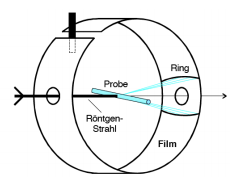
\includegraphics[width=0.4\textwidth]{aufbau.PNG}\\
		\footnotesize\sffamily\textbf{Quelle:} Praktikumsprotokolle \cite{protokoll1}
	\end{tabular}
	\caption{Versuchsaufbau}
    \label{fig:aufbau}
\end{figure}
Die gründlich gemörserte Pulverprobe wird in Glaskapillare gefüllt, welche in einem Messingträger befestigt werden, der zur Zentrierung der Pulverprobe in der Kammer, in einen Goniometerkopf eingebaut wird. Zur genauen Zentrierung steht ein Justiermikroskop zur Verfügung, das den Goniometerkopf und den Unterteil der Kamera zeigt.\\ \\
Auf den Kammerboden ist ist von außen ein Motor montiert, der während der Röntgenbestrahlung die Pulverprobe kontinuierlich dreht. Diese Rotierung soll eine bessere Gleichverteilung der Orientierung der Kristalle ermöglichen.
\section{Durchführung des Versuchs}
Das zu untersuchende Kristall war Kupfer (\ce{Cu}).\\ \\
Zunächst wurde die Probe vorbereitet, indem wir das Pulver so lange zerkleinerten, bis eine Kristallgröße von ca. $\unit[10]{\mu m}$ anzunehmen war. Dazu wurde es mit einem Stößel verfeinert und mit Vaseline an eine dünne Glasfaser geklebt. Die Glasfaser wurde in den Probehalter mit Goniometerkopf gespannt und so ausgerichtet, dass die Drehung möglichst parallel zur Drehachse verweilte. Damit sollte eine möglichst zentrahle Röntgenbestrahlung der Probe erreicht werden. Wir ließen die Probe für ca. 10 Minuten um die Probe trocknen.\\ \\
Im Film wurden, den Anforderungen der Straumanis-Technik nach, zwei Löcher im Abstand $\unit[9]{cm}$ voneinander für jeweils ein- und austretende Strahlen gestanzt.\\ \\
Daraufhin legten wir in der Dunkelkammer unter indirektem Rotlicht den Film in die Debye-Scherrer-Aufnahmekamera ein, bauten die Probe in der Kammer ein und verschließten das Ganze lichtdicht.\\ \\
Anschließend wurde die Probe für 60 Minuten mit Röntgenstrahlen der Länge $\unit[1.5418]{\angstrom}$ bestrahlt.
\section{Auswertung}
\subsection{Auswertetabelle}
Zum Indizieren des Pulverdiagramms mithilfe der Auswertetabelle sind wir folgendermaßen vorgegangen:\\ \\
Zunächst wurden die relativen Intensitäten der Beugungslinien auf einer Skala von 1 (stark) bis 5 (schwach) identifiziert (Spalte $I_{rel}$ in Tabelle \ref{tab:auswertetabelle}).\\ \\
Dann wurde die Lage der Beugungskreise im Film gemessen, die bereits im Labor mithilfe einer Filmauswertevorrichtung erfolgte, das aus einer über eine beleuchtete Glassplatte bewegliche Lupe bestand. Sie wurde über eine Millimeter-Skala bestimmt. Der Mittelpunkt der Beugungskreise wurde indirekt berechnet, da dieser in einem Loch liegt: wir maßen die Position des Kreises zu beiden Seites des Loches (Spalte $l$ und $r$) und nahmen deren Mittelwert als seinen Mittelpunkt (Spalte $\frac{1}{2}(r+l)$).\\ \\
Weiter bestimmten wir die Öffnungswinkel $2 \theta$. Die Kamera hatte einen Durchmesser $D=\unit[57.3]{mm}$, was einem Umfang von $\unit[180]{mm}$. Der Film war ebenfalls $\unit[180]{mm}$ breit, d.h. $\unit[1]{^{\circ}}$ entspricht $\unit[1]{mm}$ auf dem ausgerollten Film:
\begin{equation}
2\theta=r-l \quad \text{bzw. für Rückstreubereich (rechte Filmhälfte)} \quad 2 \theta=\unit[180]{^\circ} - (r-l)
\end{equation}
Dabei sollte auch die Filmschrumpfung, die beim Entwickeln und Trocknen des Films entstehen kann, berücksichtigt und die Öffnungswinkel entsprechend korrigiert werden. Dazu maßen wir die Breite des Films, die normalerweise $\unit[180]{mm}$ beträgt und erhielten $\approx \unit[178]{mm}$, was einer Schrumpfung um $\unit[1.11]{\%}$ entspricht. Die Schrumpfung könnte auch anhand des Mittelpunktabstandes der Beugungskreise berechnet werden, die \unit[90]{mm} betragen soll, und durch Differenz der jeweils gemittelten $\frac{1}{2}(r+l)$-Werte zu \unit[89.97]{mm} bestimmt wurde.\\ \\
Die Werte der Öffnungswinkel wurden in Tabelle \ref{tab:auswertetabelle} entsprechend korrigiert.
\begin{sidewaystable}
\begin{tabular}{|c|c|c|c|c|c|c|c|c|c|c|c|c|}
\hline
Nr & $I_{rel}$ & links [mm] & rechts [mm] & $\frac{1}{2}(r+l)$ [mm] & $2 \theta$ [$^{\circ}$] & $\sin^2{\theta_{exp}}$ & $\frac{\sin^2{\theta_n}}{\sin^2{\theta_1}}$ & $\approx h^2+k^2+l^2$ & $h^2+k^2+l^2$ & hkl & M & a [$\angstrom$]\\
\hline
1 & ss & 15.8 & 59.5 & 37.65 & 43.2 & 0.136 & 1.00 & 3.00 & 3 & 111 & 8 & 3.63 \\
2 & m & 12.0 & 63.0 & 37.50 & 50.4 & 0.182 & 1.34 & 4.02 & 4 & 200 & 6 & 3.62 \\
3 & w & 0.00 & 74.8 & 37.40 & 74.0 & 0.362 & 2.67 & 8.01 & 8 & 220 & 12 & 3.62 \\
4 & s & 82.5 & 172.5 & 127.50 & 91.0 & 0.509 & 3.75 & 11.25 & 11 & 311 & 24 & 3.59 \\
5 & w & 85.2 & 169.8 & 127.50 & 96.3 & 0.555 & 4.09 & 12.28 & 12 & 222 & 8 & 3.58 \\
6 & vw & 96.2 & 158.8 & 127.50 & 118.1 & 0.735 & 5.42 & 16.27 & 16 & 400 & 6 & 3.60 \\
7 & vw & 106.2 & 148.8 & 127.50 & 137.9 & 0.867 & 6.39 & 19.18 & 19 & 331 & 24 & 3.60 \\
8 & s & 105.8 & 149.0 & 127.40 & 137.3 & 0.871 & 6.42 & 19.26 & 19 & 331 & 24 & 3.52 \\
9 & s & 110.0 & 145.0 & 127.50 & 145.4 & 0.911 & 6.72 & 20.16 & 20 & 420 & 24 & 3.62 \\
10 & vw & 110.5 & 144.5 & 127.50 & 146.4 & 0.916 & 6.76 & 20.27 & 20 & 420 & 24 & 3.60 \\
\hline
\end{tabular}
\caption{Auswertetabelle für Debye-Scherrer-Aufnahmen (Straumanis-Technik)}
\label{tab:auswertetabelle}
\end{sidewaystable}
Aus der Braggschen-Gleichung
\begin{equation*}
n \cdot \lambda = 2d \sin \theta
\end{equation*}
und der Abhängigkeit des Netzebenenabstandes $d$ von den Millerschen Indizes $h$, $k$, $l$
\begin{equation*}
d=\frac{a}{\sqrt{h^2+k^2+l^2}}
\end{equation*}
folgt:
\begin{equation}
\label{eq:derivationGitterkonstante}
\frac{\lambda}{2 a}=\frac{\sin \theta}{\sqrt{h^2+k^2+l^2}}=const
\end{equation}
Es folgt weiter:
\begin{equation*}
\frac{\sin^2 \theta_2}{\sin^2 \theta_1}=\frac{h_2^2+k_2^2+l_2^2}{h_1^2+k_1^2+l_1^2}
\end{equation*}
Damit kann die Spalte $h^2+k^2+l^2$ bestimmt werden. Wir gingen so vor, dass wir dem 1. Ring eine geeignete ganze Zahl für $h^2+k^2+l^2$ zuwiesen, sodass für die nachfolgenden Ringe für $h^2+k^2+l^2$ aus dem Verhältnis $\frac{\sin^2 \theta_n}{\sin^2 \theta_1}$ sich ebenfalls eine ganze Zahl ergeben hat.\\ \\
Die Gitterkonstante ergibt sich aus Gleichung \ref{eq:derivationGitterkonstante}:
\begin{equation*}
a=\sqrt{\frac{\lambda^2 \cdot (h^2+k^2+l^2)}{4 \sin^2{\theta}}}
\end{equation*}
wobei $\lambda$ die Wellenlänge der Röntgenstrahlung $\lambda=\unit[1.5418]{\angstrom}$ ist.\\ \\
Der Mittelwert der Gitterkonstanten $\overline{a}$ und der Fehler $\sigma_a$ (Standardabweichung) betragen jeweils:
\begin{equation*}
\overline{a}=\unit[3.60]{\angstrom} \quad \quad \sigma_a=\unit[0.03]{\angstrom}
\end{equation*}
Bei der Bestimmung von $a$ sollen die Aufspaltungen von $K \alpha_1$ (\unit[1.54051]{\angstrom}) und $K \alpha_2$ (\unit[1.54433]{\angstrom}) berücksichtigt werden.\\ \\
Unsere berechnete Gitterkonstante $a$ hat einen sehr guten Wert, denn sie liegt recht nah am reelle Wert von Kupfer \ce{Cu} mit \unit[3.61]{\angstrom}. Das macht sich auch am sehr kleinen Fehler bemerkbar.\\ \\
Das Volumen der Elementarzelle erhält man aufgrund der kubischen Elementarzelle einfach aus $V=a^3$, deren Fehler mit Fehlerfortpflanzung ergibt sich zu $\sigma_V=3 \cdot a^2 \cdot \sigma_a$:
\begin{equation*}
V=\unit[46.66]{\angstrom^3} \quad \quad \sigma_V=\unit[1.17]{\angstrom^3}
\end{equation*}
\subsection{Zahl der Formeleinheiten in der Elementarzelle}
Die Zahl der Formeleinheiten $Z$ in der Elementarzelle gibt an, wie viele Atome oder Ionen in der Elementarzelle hineinpassen. Sie wird laut Vorbereitungsmappe wie folgt bestimmt:
\begin{equation*}
Z=\frac{d_m \cdot V \cdot N_A}{M}
\end{equation*}
wobei 
\begin{itemize}
\item $d_m=\unit[8.92]{g/cm^3}$ die experimentell bestimmte Dichte von \ce{Cu}
\item $M=\unit[63.55]{g/mol}$ die molare Masse von \ce{Cu}
\item $V=\unit[46.66]{\angstrom^3}=\unit[46.90 \cdot 10^{-24}]{cm^3}$ das zuvor bestimmte Volumen der Elementarzelle
\item $N_A=\unit[6.022 \cdot 10^{23}]{mol^{-1}}$ die Avogadro-Zahl
\end{itemize}
Wir erhalten $Z=3.94 \approx 4$. Die Anzahl der Atome pro Elementarzelle beträgt damit $4$.
\subsubsection{Bravais-Gitter}
Die im Pulverdiagramm fehlenden $hkl$-Reflexe sind alle möglichen $hkl$-Reflexe abzüglich der in der Auswertetabelle \ref{tab:auswertetabelle} identifizierten. Sie sind in Tabelle \ref{tab:fehlendereflexe} aufgelistet.
\begin{longtable}[H]{c||c||c||c}
hkl&hkl&hkl&hkl\\
\hline
100 & 441 & 421 & 621\\
110 & 521 & 332 & 541\\
210 & 433 & 422 & 533\\
211 & 530 & 430 & 622\\
221 & 531 & 500 & 542\\
300 & 442 & 431 & 630\\
310 & 600 & 510 & 631\\
320 & 610 & 333 & 444\\
321 & 532 & 511 & 632\\
322 & 611 & 432 & 700\\
410 & 620 & 520 & 543\\
330 & 443 & 521 & 550\\
411 & 540 & 440 & 710\\
\caption{Im Pulverdiagramm fehlende Reflexe}
\label{tab:fehlendereflexe}
\end{longtable}
Die Bestimmung des Bravais-Gitters erfolgt mithilfe der Bedigungen für integrale Auslöschungen. Die Existenz von systematischen Auslöschungen weist man anhand der in Seite 19 der Vorbereitungsmappe aufgeführten Auslöschungsregeln und der in der Auswertetabelle bestimmten Millerschen-Indizes $hkl$ nach.\\ \\
Alle bestimmten $hkl$ erfüllen folgende Bedingungen:
\begin{align*}
h+k& = 2n\\
h+l& = 2n\\
k+l& = 2n
\end{align*}
Somit erfüllen die fehlenden Reflexe die Bedingungen:
\begin{align*}
h+k& \neq 2n\\
h+l& \neq 2n\\
k+l& \neq 2n
\end{align*}
Diese Bedingungen entsprechen den Bedingungen für integrale Auslöschungen verursacht durch ein F- (kubisch flächenzentriertes) Gitter. Es treten auch zonale und seriale Auslöschungen auf.\\ \\
Diese Ergebnisse weisen darauf hin, dass die Kupferprobe ein kubisch flächenzentriertes (fcc) Bravais-Gitter hat.
\subsection{Strukturvorschläge}
Es sollen nun Strukturvorschläge anhand der Ionenradien und der Koordinationszahlen gemacht werden. Im Fall von Kupfer befinden sich in den Elementarzellen keine Ionen sondern nur \ce{Cu}-Atome. Wenn wir annehmen, dass das Kristall eine fcc-Gitter-Struktur aufweist, so befinden sich die 4 \ce{Cu}-Atome pro Elementarzelle in jedem Gitterpunkt.\\ \\
Die Punktlagen der \ce{Cu}-Atome in der Elementarzelle sind:
\begin{equation*}
(0,0,0) \quad (1, 1, 0) \quad (1,0,1) \quad (0,1, 1)
\end{equation*}
Wenn wir weiter annehmen, dass das Kristall eine dichteste Kugelpackung ist, so befinden sich in den Tetra- und Oktaederlücken keine Atome.
\subsection{Strukturfaktorausdruck}
Nun soll für die bisher gemachten Strukturvorschläge der Strukturfaktorausdruck nach Gleichung \ref{eq:strukturfaktor} entwickelt und mit den beobachteten Intensitäten im Film verglichen werden.\\ \\
Einsetzen der Punktlagen der Atome in den Strukturfaktor ergibt:
\begin{equation*}
F(hkl)=f_{\ce{Cu}} \cdot (1 + e^{2 \pi i (h+k)} + e^{2 \pi i (h + l)} + e^{2 \pi i (k + l)})
\end{equation*}
mit $f_{\ce{Cu}}$ der Formfaktor des $\ce{Cu}$-Atoms. Für die komplexe Exponentialfunktion gilt folgende Äquivalenz:
\begin{equation*}
e^{ix}=\cos{(x)} + i \sin{(x)}
\end{equation*}
Daher wird $e^{i 2 \pi n}=1$ für gerade $n$ und für ungerade $n$ $e^{i 2 \pi n}=-1$.\\ \\
Je nachdem, ob die jeweiligen Indizes $hkl$ gerade oder ungerade sind, ergibt sich wir für den Strukturfaktor $F(hkl)$ folgende Fallunterscheidung:
\begin{itemize}
\item $F(hkl)=4 \cdot f_{\ce{Cu}}$, falls alle Indizes $hkl$ gerade sind
\item $F(hkl)=4 \cdot f_{\ce{Cu}}$, falls alle Indizes $hkl$ ungerade sind
\item $F(hkl)=0$ sonst
\end{itemize}
Die Ergebnisse, die wir durch den Strukturfaktor erhalten, stimmen mit den Auslöschungsregeln überein. Wir erhielten Reflexe erst, wenn die Summen $h+l$, $h+l$ und $k+l$ gerade waren, was der Fall ist, wenn entweder alle Indizes gerade oder ungerade aber nicht gemischt sind.\\ \\
Vergleicht man die Intensitäten mit den Indizes $hkl$, so erkennt man keinen Zusammenhang. Die Intensitäten sind unterschiedlich. Eigentlich müssten, laut dem bestimmten Strukturfaktor, alle Intensitäten gleich sein, unabhängig davon, ob die Millerschen Indizes in der Tripel gerade oder ungerade sind. Es muss jedoch beachtet werden, dass die Intensitäten mit dem Auge bestimmt wurden und damit ungenau sind.
\subsection{Kürzeste Atomabstände}
Abbildung \ref{fig:cu-elementarzelle} zeigt eine Projektion des Elementarzellinhalts der Kristallstruktur.
\begin{figure}[H]
	\centering
	\begin{tabular}{@{}r@{}}
		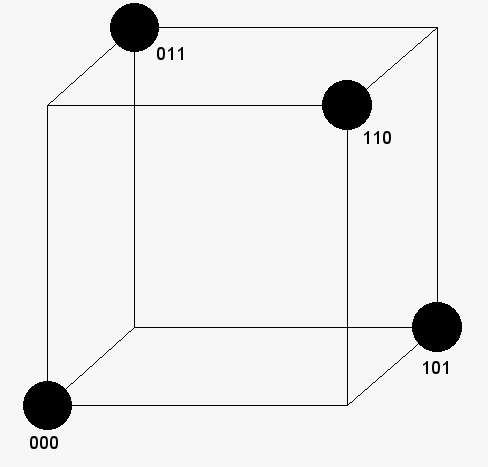
\includegraphics[width=0.35\textwidth]{cu-elementarzelle.png}\\
		\footnotesize\sffamily\textbf{Quelle:} Selbst gezeichnet
	\end{tabular}
	\caption{Projektion der \ce{Cu}-Atome in der Elementarzelle}
    \label{fig:cu-elementarzelle}
\end{figure}
Abbildung \ref{fig:cu-kristall} zeigt die Kristallstruktur, die durch die unendliche Verschiebung der Elementarzelle aus Abbildung \ref{fig:cu-elementarzelle} entsteht.
\begin{figure}[H]
	\centering
	\begin{tabular}{@{}r@{}}
		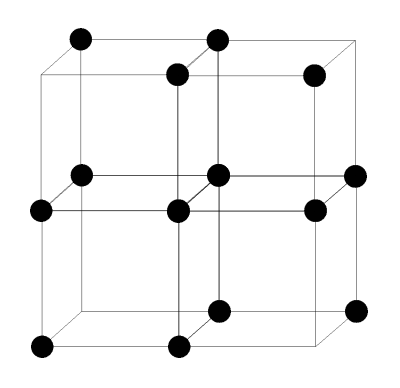
\includegraphics[width=0.35\textwidth]{cu-kristall.png}\\
		\footnotesize\sffamily\textbf{Quelle:} Selbst gezeichnet
	\end{tabular}
	\caption{Struktur des Kupferkristalls}
    \label{fig:cu-kristall}
\end{figure}
Wie man in Abbildung \ref{fig:cu-kristall} sehen kann, betragen die Koordinationszahlen der einzelnen Atome 6. Aus dieser Abbildung folgt auch, dass alle Atome im Kristall denselben Abstand haben. Dieser Abstand entspricht der halben Gitterkonstante $a$:
\begin{equation*}
s=\frac{1}{2} a
\end{equation*}
Der entsprechende Fehler $\sigma_s$ ergibt sich mit Fehlerfortpflanzung zu:
\begin{equation*}
\sigma_s= \frac{\partial s}{\partial a} \sigma_a=\frac{1}{2} \sigma_a
\end{equation*}
Damit ergibt sich für den kürzesten Atomabstand im Kristall der Wert:
\begin{equation*}
\sigma_s=\unit[(1.800 \pm 0.015)]{\angstrom}
\end{equation*}
\section{Änderungsprotokoll}
\begin{table}[H]
\centering
\begin{tabularx}{\textwidth}{| c | c | X |}
\hline
\textbf{Datum} & \textbf{Abschnitt} & \textbf{Details}\\
\hline
06. Februar 2015 & - & 1. Fassung\\
\hline
\end{tabularx}
\end{table}
\bibliographystyle{acm}
\bibliography{literatur}

\end{document}